\section{Resultados Experimentais}

\begin{description}

\item{\textbf{\textit{Latency} / \textit{Bandwidth}:}}
As interacções do cliente com o sistema são feitas a partir da biblioteca \textbf{PADI-DSTM}. De seguida seguem o número de mensagens trocadas durante os vários tipos de interacção e por último, os resultados concretos recolhidos no exemplo Circle.cs (2 clientes concorrentes e 3 servidores). Note-se que a mensagem de maior tamanho é a que transporta o PadInt serializável, tendo um tamanho que depende do número de \textit{tries}. De um modo genérico, as mensagens trocadas são as seguintes:

\begin{itemize}
\item \textbf{TxBegin}\\
1. Cliente $\longleftrightarrow$ Master\\
2. Cliente $\longleftrightarrow$ Coordenador

\item \textbf{TxCreate / TxAccess / Read / Write}\\
1. Cliente $\longleftrightarrow$ Coordenador\\
2.(Coordenador $\longleftrightarrow$ Master)\footnote{\label{note1}Apenas se a informação não estiver em cache.}\\
3. Coordenador $\longleftrightarrow$ Servidor [primário]\\
4.(Servidor [primário] $\longleftrightarrow$ Master)\footnotemark[2]\\
5. Servidor [primário] $\longleftrightarrow$ Servidor [replicado]

\item \textbf{TxCommit}\\
Durante esta fase é chamado o PrepareCommit, se tudo correr bem é chamado o Commit, caso contrário é chamado o Abort. As mensagens trocadas durante o Prepare para cada PadIint da transacção são as seguintes:\\[0,05in]
1. Cliente $\longleftrightarrow$ Coordenador\\
2.(Coordenador $\longleftrightarrow$ Master)\footnotemark[2]\\ 
3. Coordenador $\longleftrightarrow$ Servidor [primário]\\
4.(Servidor [primário] $\longleftrightarrow$ Master)\footnotemark[2]\\
5. Servidor [primário] $\longleftrightarrow$ Servidor [replicado]\\[0,05in]
As mensagens trocadas durante o Commit propriamante dito são as seguintes:\\[0,05in]
1. Coordenador $\longleftrightarrow$ Servidor [primário]\\
2. Servidor [primário] $\longleftrightarrow$ Servidor [replicado]\\[0,05in]
Dado que o Abort pode ser chamado durante um commit, devido à falta de sucesso na preparação dos PadInts, o número de mensagens trocadas nesta fase vai depender do número de PadInts e da preparação com sucesso dos mesmos.

\item \textbf{TxAbort}\\
O TxAbort é semelhante ao TxCommit, excluindo as mensagens de Prepare.
\end{itemize}

\begin{figure}[htb]
\centering
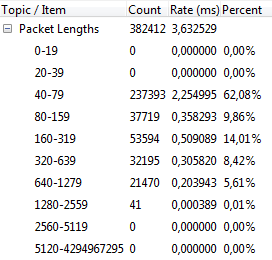
\includegraphics[width=0.3\textwidth]{packet.png}
\caption{\label{fig:packet}Estatísticas do exemplo Circle.cs (com 2 clientes concorrentes e 3 servidores).}
\end{figure}

\item{\textbf{\textit{Parallel progress allowed in transaction}}:}
Pela análise experimental verificamos que, mesmo com o mecanismo em que as transacções esperam por outras transacções ,que necessitam para fazerem \textit{commit}, a ordem de término de execução dos clientes segue a ordem de entrada dos mesmos no sistema. Isto é, no conjunto de clientes, a execução é sequencial, sendo que para transacções dentro do mesmo intervalo numérico de instruções, os primeiros clientes a iniciarem transacções normalmente também são os primeiros a terminarem. Também foi raro o caso em que o mesmo PadInt foi modificado no mesmo intervalo de tempo por mais de uma transacção (\textit{tries}), por isso existiu um elevado paralelismo, mas caso o mesmo PadInt seja modificado por várias transacções diferentes que façam \textit{commit} por ordem diferente da ordem de chegada ao sistema,  o número de \textit{aborts} aumenta bastante. Este tipo de situação pode levar a uma diminuição bastante significativa da \textit{performance}.

\item{\textbf{\textit{Throughput}:}} 
Em média, com testes feitos num intervalo de 1 a 10 clientes, a média foi de 30 transacções por segundo.  Note-se que o número de instruções de cada transação foi gerado aleatoriamente num intervalo de 1 a 100 e as próprias instruções são escolhidas de forma aleatória, isto é, \textit{create} aleatório de um PadInt ainda não existente, \textit{access} aleatório de um PadInt já criado e \textit{read}/\textit{write} de um PadInt já acedido. Deste modo, o número máximo de \textit{creates} que podem ser feitos fica limitado pelo PadInt com maior valor, e podem nem sempre ser todos criados, porque tal como já foi referido, as operações executadas são geradas segundo um valor aleatório. Concluímos que 95\% das transacções fizeram \textit{commit} com sucesso, sendo um resultado bastante aceitável.

\begin{table}[htb]
\centering
\begin{tabular}{c|c|c|c}
 & Nr. de & & \\
 Nr. de& transacções &  Nr. de & Nr. de \\
clientes & por cliente & PadInts & servidores \\\hline
5 & 500 & 2 & 5\\
5 & 500 & 5 & 5\\
5 & 1 000 & 100 & 5\\
5 & 2 000 & 200 & 5\\
10 & 2 000 & 2 147 483 647 & 5\\
\end{tabular}
\caption{\label{tab:throughput}Dados usados na análise de \textbf{\textit{throughput}}.}
\end{table}

\item{\textbf{\textit{Load balancing regarding data storage and processing among servers}}:}
Pelos testes referidos na tabela abaixo verificou-se que quando a migração não está activa, o resultado obtido em média foi Servidor 1 (24\%), Servidor 2 (16\%), Servidor 3 (35\%), Servidor 4 (11\%), Servidor 5 (14\%), o que até se verificou bastante aceitável, tendo em conta que o algoritmo é puramente aleatório entre os servidores disponíveis.

Com a migração activa conseguiu-se obter resultados muito melhores, sendo estes em media: Servidor 1 (21\%), Servidor 2 (18\%), Servidor 3 (20\%), Servidor 4 (19\%), Servidor 5 (22\%).

\begin{table}[htb]
\centering
\begin{tabular}{c|c|c|c|c|c}
\textbf{Nr. de PadInts} &  \textbf{S1} &  \textbf{S2} & \textbf{S3} & \textbf{S4} & \textbf{S5} \\\hline
2 & 1 & 1 & 0 & 0 & 0\\
5 & 1 & 1 & 1 & 1 & 1\\
100 & 16 & 21 & 26 & 19 & 18\\
200 & 26 & 54 & 32 & 48 & 40\\
2 147 483 647 & 125 & 109 & 93 & 141 & 117\\
\end{tabular}
\caption{\label{tab:balanceamento}Número de PadInts por servidor.}
\end{table}

\item{\textbf{\textit{Lost updates} / \textit{Inconsistent retrievals} / \textit{Proneness to deadlocks}:}} 
Não experienciamos qualquer evento deste tipo mas pensamos que existem casos em que podem ocorrer se o sistema estiver completamente sobrecarregado. Em parte, pode ser explicado pela nossa abordagem de TimeStamp Ordering\cite{ex1} que mantém uma ordem de acesso universal aos dados, mantendo a consistência dos mesmos e evitando a presença de \textit{deadlocks}.

\item{\textbf{\textit{Amount of aborted transactions} / \textit{Proneness to cascading aborts}:}} 
Em média o nosso sistema aborta 5\% do total das transacções, devido a \textit{cascading aborts}. Isto acontece porque são verificadas as dependências das transacções que estão prestes a fazer \textit{commit}, caso precisem de esperar pelo resultado de outras que ainda não o tenham feito. Isto é bom se as transacções pelas quais estamos à espera tenham sucesso, caso contrário dá-se um \textit{cascading abort}. Pelos resultados obtidos concluímos que esta foi a melhor abordagem a aplicar, porque o número de transacções abortadas é bastante pequeno. Tome-se por excepção o caso em que vários clientes acedem, ao mesmo tempo, ao mesmo PadInt, porque nesse caso o número de transacções abortadas aumenta para mais de metade, mas é extremamente raro existirem clientes suficientes num dado instante de modo a que isto aconteça.

\end{description}